% Created with jtex v.1.0.3
\documentclass{article}
\usepackage{arxiv}

\usepackage[utf8]{inputenc} % allow utf-8 input
\usepackage[T1]{fontenc}    % use 8-bit T1 fonts
\usepackage{hyperref}       % hyperlinks
\usepackage{url}            % simple URL typesetting
\usepackage{datetime}       % show dates in the title block
\usepackage{booktabs}       % professional-quality tables
\usepackage{amsfonts}       % blackboard math symbols
\usepackage{nicefrac}       % compact symbols for 1/2, etc.
\usepackage{microtype}      % microtypography
\usepackage{graphicx}
\usepackage{natbib}
\usepackage{doi}
\usepackage{xcolor}

%%%%%%%%%%%%%%%%%%%%%%%%%%%%%%%%%%%%%%%%%%%%%%%%%%
%%%%%%%%%%%%%%%%%%%%  imports  %%%%%%%%%%%%%%%%%%%
\usepackage{amsmath}
%%%%%%%%%%%%%%%%%%%%%%%%%%%%%%%%%%%%%%%%%%%%%%%%%%

\hypersetup{colorlinks = true,
linkcolor = purple,
urlcolor  = blue,
citecolor = cyan,
anchorcolor = black}

\title{The attractor states of the functional brain connectome}

\newdate{articleDate}{14}{7}{2023}
\date{\displaydate{articleDate}}

\makeatletter
\let\@fnsymbol\@arabic
\makeatother

\author{Robert Englert\\
University Medicine Essen\\\AND
Tamas Spisak\footnotemark[1]\\
University Medicine Essen\\}

% Uncomment to override  the `A preprint' in the header
\renewcommand{\headeright}{Preprint}
\renewcommand{\undertitle}{}
\renewcommand{\shorttitle}{ConnAttractor Preprint}

%% Add PDF metadata to help others organize their library
%% Once the PDF is generated, you can check the metadata with
%% $ pdfinfo template.pdf
\hypersetup{
pdftitle={\@title},
pdfsubject={},
pdfauthor={\@author},
pdfkeywords={},
addtopdfcreator={Written in Curvenote}
}

\begin{document}
\maketitle
\footnotetext[1]{Correspondence to: tamas.spisak@uk-essen.de}

\begin{abstract}
\textbf{Abstract:}

todo
\end{abstract}

\keywords{}

\textbf{Key Points:}

\begin{itemize}
\item We propose a high-level computational model of "activity flow" across brain regions
\item The model considers the funcional brain connectome as an already-trained Hopfield neural network
\item It defines an energy level for any arbitrary brain activation patterns
\item and a trajectory towards one of the finite number of stable patterns (attractor states) that minimize this energy
\item The model reproduces and explains the dynamic repertoir of the brain's spontanous activity at rest
\item It conceptualizes both task-induced and pathological changes in brain activity as a shift on the "attractor landscape"
\item We validate our findings on healthy and clinical samples ({\textasciitilde}2000 participants)
\end{itemize}

\section{Introduction}\label{Introduction}

Brain function is characterized by the continuous activation and deactivation of anatomically distributed neuronal populations.
While the focus of related research is often on the direct mapping between changes in the activity of a single brain area and a specific task or condition, in reality, regional activation never seems to occur in isolation (\cite{Bassett_2017}).
Regardless of the presence or absence of explicit stimuli, brain regions seem to work in concert, resulting in a rich and complex spatiotemporal fluctuation (\cite{Gutierrez_Barragan_2019}).
This fluctuation is neither random, nor stationary over time \cite{Liu_2013}; \href{https://doi.org/10.1073/pnas.1400181111}{}. It shows quasi-periodic properties (\cite{Thompson_2014}), with a limited number of recurring patterns known as ``brain states'' (\href{https://doi.org/10.1016/j.tins.2023.04.001}{}; \href{https://doi.org/10.1073/pnas.1705120114}{}; \href{https://doi.org/10.1073/pnas.1216856110}{}; \href{https://doi.org/10.1016/j.neuroimage.2010.05.081}{}).

Whole-brain dynamics have previously been characterized with various descriptive techniques (\href{https://doi.org/10.1073/pnas.1121329109}{}; \cite{Vidaurre_2017}; \href{https://doi.org/10.1073/pnas.1216856110}{}; \cite{Chen_2018}), providing accumulating evidence not only for the existence, but also for the high neurobiological and clinical significance, of such dynamics (\href{https://doi.org/10.1016/j.neuroimage.2013.05.079}{}; \href{https://doi.org/10.1073/pnas.1418031112}{}; \cite{Meer_2020}). However, due to the nature of such studies, the underlying driving forces remain elusive.

% Brain state dynamics can be assessed with multiple techniques, dynamic connectivity analysis (), including independent component analysis ([](https://doi.org/10.1073/pnas.1121329109)), hidden markov models ([](https://doi.org/10.1073/pnas.1705120114)) or point-process analyses to capture co-activation patterns (CAPs, [](https://doi.org/10.1073/pnas.1216856110); [](https://doi.org/10.1016/j.neuroimage.2015.01.057); [](https://doi.org/10.3389/fnsys.2013.00101); [](https://doi.org/10.1038/s41467-020-18717-w)), clustering [](10.1089/brain.2018.0586)

Questions regarding the mechanisms that cause these remarkable dynamics can be addressed through computational models, which have the potential to shift our understanding from mere associations to causal explanations.
Conventional computational approaches try to solve the puzzle by delving all the way down to the biophysical properties of single neurons and then aim to construct a model of larger neural populations, or even the entire brain (\href{https://doi.org/10.1038/nn.4497}{}).
While such approaches have demonstrated numerous successful applications (\cite{Kriegeskorte_2018}; \href{https://doi.org/10.1093/schbul/sby154}{}), the estimation of all the free parameters in such models presents a grand challenge. This limitation hampers the ability of these techniques to effectively bridge the gap between explanations at the level of single neurons and the complexity of behavior (\href{https://doi.org/10.1038/nn.4497}{}).

An alternative approach, known as "neuroconnectomism" (\href{https://doi.org/10.1038/s41583-023-00705-w}{}) shifts the emphasis from "biophysical fidelity" of models to "cognitive/behavioral fidelity" (\href{https://doi.org/10.1038/s41593-018-0210-5}{}), by using artificial neural networks (ANNs) that were trained to perform various tasks, as brain models.
While this novel approach has already significantly contributed to expanding our understanding of the general computational principles of the brain (see \href{https://doi.org/10.1038/s41583-023-00705-w}{}), the requirement of training ANNs for specific tasks poses inherent limitations in their capacity to explain the spontaneous macro-scale dynamics of neural activity (\href{https://doi.org/10.1038/s41593-019-0520-2}{}).

In this work, we adopt a middle ground between traditional computational modeling and neuroconnectionism to investigate the phenomenon of brain dynamics.
On one hand, similar to neuroconnectionism, our objective is not to achieve a comprehensive bottom-up understanding of neural mechanisms. Instead, we utilize an artificial neural network (ANN) as a high-level computational model of the brain (Figure~\ref{concept}A).
On the other hand, we do not train our ANN for a specific task. Instead, we empirically set its weights based on  data about the "activity flow" (\href{https://doi.org/10.1038/nn.4406}{}; \href{https://doi.org/10.1038/s41467-017-01000-w}{}) across regions within the functional brain connectome, as measured with functional magnetic resonance imaging (fMRI, Figure~\ref{concept}B).
We employ a neurobiologically motivated ANN architecture, a continuous-space Hopfield network (\href{https://doi.org/10.1073/pnas.79.8.2554}{}; \href{https://doi.org/10.1038/s42254-023-00595-y}{}).

Within this architecture, the topology of the functional connectome naturally defines an energy level for any arbitrary activation patterns and a trajectory towards one of the finite number of stable patterns that minimize this energy, the so-called attractor states.
Our model also offers a natural explanation for brain state dynamics.
In the presence of weak noise, the system does not converge into an equilibrium state but undergoes "bifurcation", enabling it to traverse extensive regions of the state space, moving on a path restricted by the "gravitational pull" of different attractor states (Figure~\ref{concept}C).

\begin{figure}[!htbp]
\centering
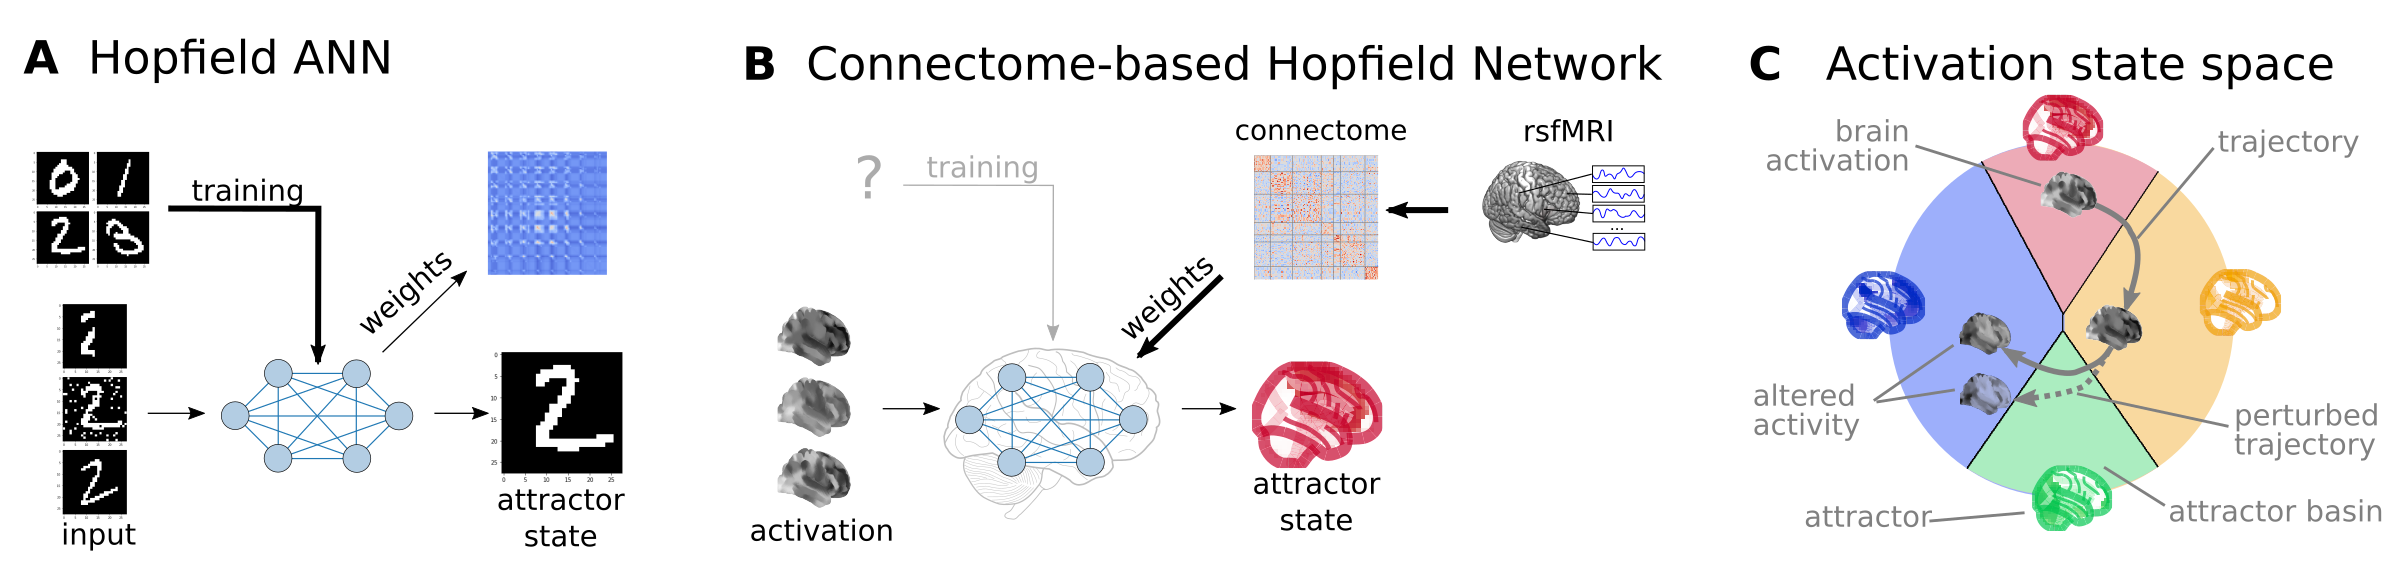
\includegraphics[width=0.7\linewidth]{files/concept-8ef5485a6935c62c94405b501ac09d92.png}
\caption[]{\textbf{Connectome-based Hopfield networks as models of macros-scale brain dynamics.} \newline
\newline

\textbf{A)} Hopfield artificial neural networks (ANNs)  are a form of recurrent ANNs that serve as content-addressable ("associative") memory systems. Hopfield networks can be trained to store a finite number of patterns (e.g. via Hebbian learning). During the training procedure, the weights of the Hopfield ANN are trained so that the stored patterns become stable attractor states of the network. Thus, when the trained network is presented partial or noisy variations of the stored patterns, it can effectively reconstruct the original pattern via an iterative relaxation procedure that converges to the attractor states.
\textbf{B)} Instead of training the Hopfield network to specific tasks, we use the topology of the functional brain connectome to define the weights of the Hopfield network. Following form the strong analogies between the relaxation rule of Hopfield networks and the activity flow principle that links activity to connectivity in brain networks, we propose the constructed connectome-based Hopfield network as a computational model for macro-scale brain dynamics.  \textbf{C)} The proposed computational framework assigns an energy level, an attractor state and a position in a low-dimensional embedding to brain activation patterns. Additionally, it models how the whole state-space of viable activation patterns is restricted by the dynamics of the system how alterations in activity and/or connectivity modify these dynamics.}
\label{concept}
\end{figure}

In this simplistic yet powerful framework, both spontaneous and task-induced brain dynamics can be conceptualized as a high-dimensional path that meanders on the reconstructed energy landscape in a way that is restricted by the "gravitational pull" of the attractors states.
The framework provides a generative model for both resting state and task-related brain dynamics, offering novel perspectives on the mechanistic origins of resting state brain states and task-based activation maps.

In the present work, we first explore the attractor states of the functional brain connectome and construct a low-dimensional representation of the energy landscape.
Subsequently, we rigorously test the proposed model through a series of experiments conducted on data obtained from 7 studies encompassing a total of n$\approx$2000 individuals.

These analyses include evaluation of robustness and replicability, testing the model's ability to reconstrcut various characteristics of resting state brain dynamics as well as its capacity to detect and explain changes induced by tasks or pathological conditions.

These experiments provide converging evidence for the validity of connectome-based Hopfield networks as models of brain dynamics and highlight their potential to provide a fresh perspective on a wide range  of research questions in basic and translational neuroscience.

\section{Results}\label{Results}

\subsection{Connectome-based Hopfield network as a model of brain dynamics}\label{Connectome-based Hopfield network as a model of brain dynamics}

First, we explored the attractor states of the functional brain connectome in a sample of n=41 healthy young participants (study 1). We estimated interregional activity flow (\href{https://doi.org/10.1038/nn.4406}{}; \href{https://doi.org/10.1038/s41467-017-01000-w}{}) as the study-level average of regularized partial correlations among the resting state fMRI timeseries of m = 122 functionally defined brain regions (BASC brain atlas, see Methods for details). We then used the standardized functional connectome as the $w_{ij}$  weights of a continuous-state Hopfield network (\href{https://doi.org/10.1073/pnas.79.8.2554}{}, \href{https://doi.org/10.1162/neco.1994.6.3.459}{}) consisting of $m$ neural units, each having an activity $a_i \in [ -1,1]$. Hopfield networks can be initialized by an arbitrary activation pattern ($m$ activations) and iteratively updated, until convergence ("relaxation"), according to the following equation:

\begin{equation}
\label{hopfield-update}
\dot{a}_i = S(\beta \sum_{j=1}^m w_{ij}a_j - b_i)
\end{equation}

where $\dot{a}_i$ is the activity of neural unit $i$ in the next iteration and $S(a_j)$ is the sigmoidal activation function $S(a) = tanh(a)$ and $b_i$ is the bias of unit $i$ and $\beta$ is the so-called temperature parameter. For the sake of simplicity, we set $b_i=0$ in all our experiments.
Importantly, in our implementation, the relaxation of the Hopfield network can be conceptualized as the repeated application of the activity flow principle, simultaneously for all regions: $\dot{a}_i = \sum_{j=1}^m w_{ij}a_j$. The update rule also exhibits strong analogies with the inner workings of neural mass models  (\href{https://doi.org/10.1038/nn.4497}{}) as applied e.g. in dynamic causal modelling (see Discussion for more details).

Hopfiled networks assign an energy to every possible activity configurations (see Methods), which decreases during the relaxation procedure until reaching an equilibrium state with minimal energy (Figure~\ref{attractors}A, top panel, \href{https://doi.org/10.1073/pnas.79.8.2554}{}; \href{https://doi.org/10.1162/neco.1994.6.3.459}{}).
We used a large number of random initializations to obtain all possible attractor states of the connectome-based Hopfield network in study 1 (Figure~\ref{attractors}A, bottom panel).

\begin{figure}[!htbp]
\centering
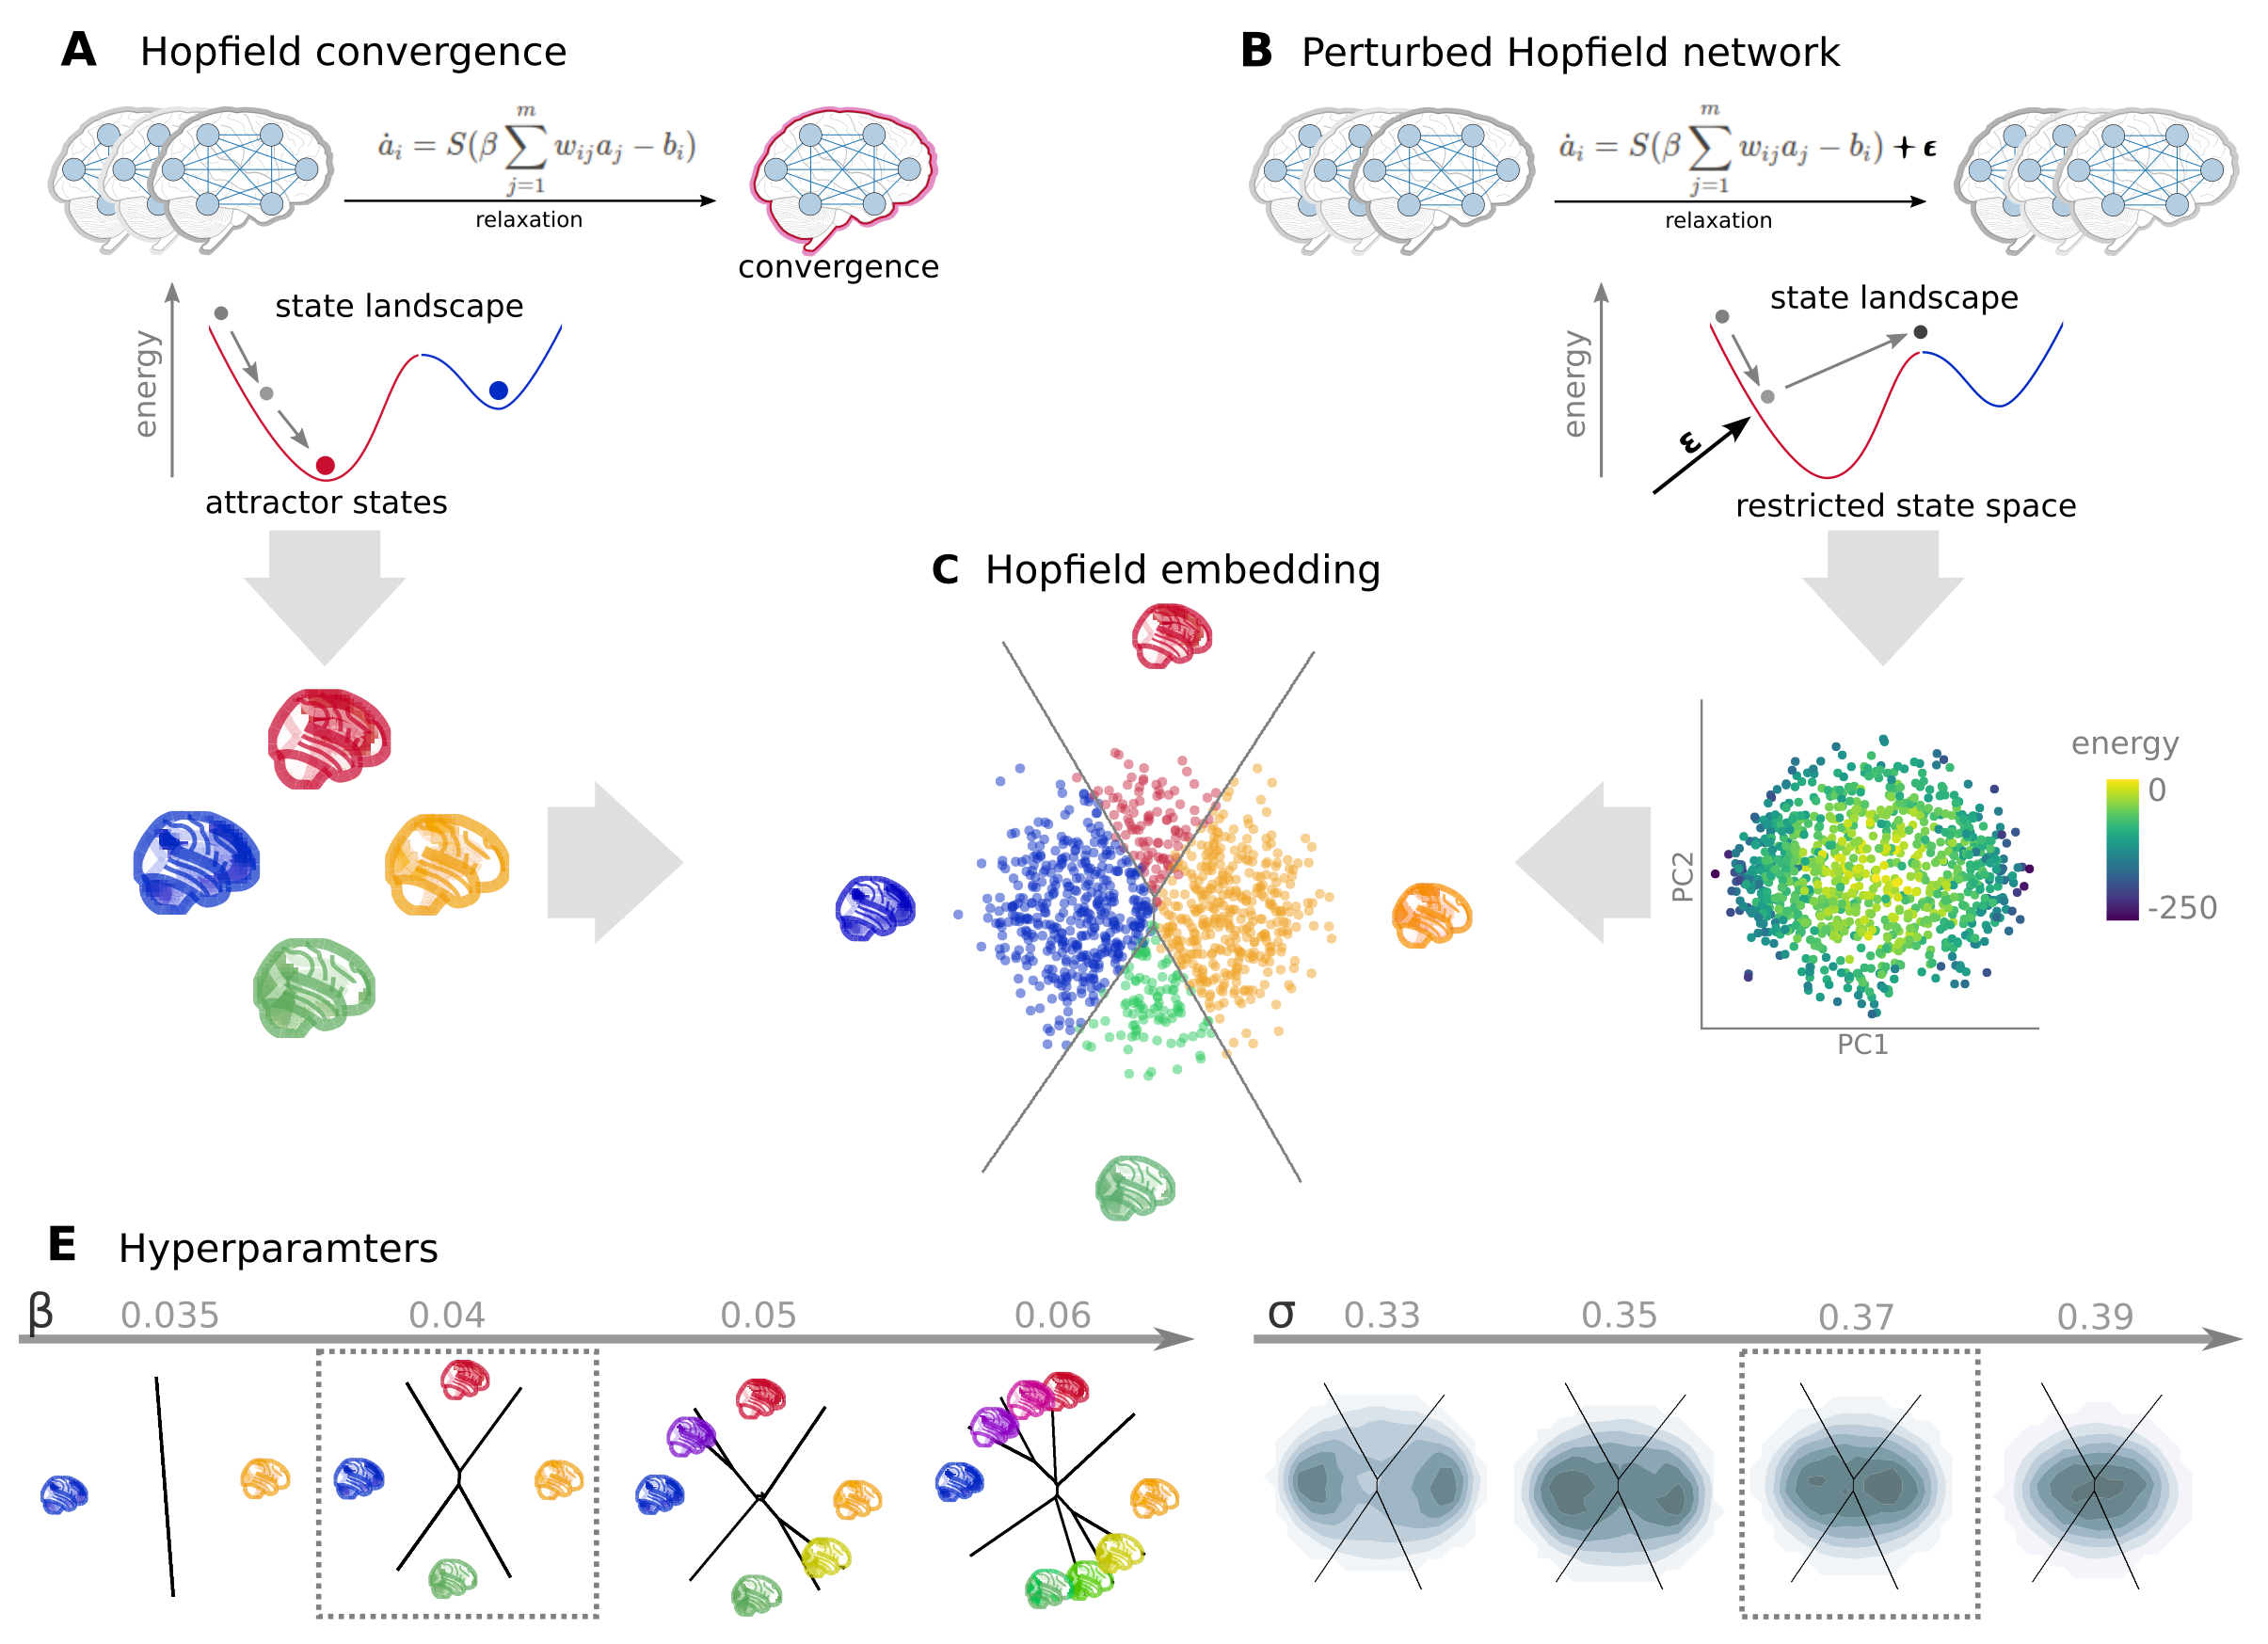
\includegraphics[width=0.7\linewidth]{files/embedding_method-883e84b8f83f7e97df2986f2e484e580.png}
\caption[]{Empirical Hopfield-networks.}
\label{attractors}
\end{figure}

We observed that, in line with theory, increasing the temperature parameter $\beta$ results in an increasing number of attractor states ((Figure~\ref{attractors}E, left) appearing in symmetric pairs (i.e. $a_i = -a_j$). For the sake of simplicity, we set $\beta=0.4$ for the rest of the paper, resulting in 4 distinct attractor states (2 symmetric pairs).

Without modifications, connectome-based Hopfield networks always converge to an equilibrium state. To account for stochastic fluctuations in neuronal activity (\href{https://doi.org/10.1098/rstb.2005.1638}{}), we add weak Gaussian noise to the connectome-based Hopfield network, to prevent the system reaching equilibrium. This approach, similarly to Stochastic DCM (\href{https://doi.org/10.1016/j.neuroimage.2012.04.061}{})), induces a "stochastic walk" of the internal state (activity pattern) of the network that may traverse extensive regions of the state space, determined by the "gravity field" (basins) of multiple attractor states (Figure~\ref{attractors}B).

We hypothesise that the resulting dynamics reflect many important characteristics of spontaneous activity fluctuations in the brain and may serve as a useful generative computational model of large scale brain dynamics. To sample the resulting state space, we obtained 100.000 iterations (starting from a random seed pattern) of the stochastic relaxation procedure with a Hopfield network initialized with the mean functional connectome in study 1 (n=44).
Next, to increase interpretability, we obtained the first two components from a principal component analysis (PCA) on the resulting state space sample to construct a low-dimensional embedding. Largely independent on the free parameter $\sigma$ (variance of the noise), the first two principal components (PCs) explained around 15\% of the variance in the state space, with low energy states (attractor states) located at the extremes of the PCs (Figure~\ref{attractors}B, bottom plot).
The PCA embedding was found to be largely consistent across different values of $\beta$ and $\sigma$ (Figure~\ref{attractors}E). For all further analyses, we fixed $\sigma=0.37$, as a result of a coarse optimization procedure to reconstruct the bimodal distribution of empirical data on the same projection (Figure~\ref{attractors}E, see Methods for details)
On the low-dimensional embedding, which we refer to as the \textit{Hopfield projection}, we observed a clear separation of the attractor states (Figure~\ref{attractors}C), with the two symmetric pairs of attractor states located at the extremes of the first and second PC.
To map the attractor basins onto the space spanned by the first two PCs (Figure~\ref{attractors}C), we obtained the attractor state of each point visited during the stochastic relaxation and fit a multinomial logistic regression model to predict the attractor state from the first two PCs. The resulting model achieved a high prediction accuracy (out-of-sample accuracy 96.5\%). Attractor bases were visualized based on the decision boundaries of this  model (Figure~\ref{attractors}C).
.We propose the Hopfield projection depicted on (Figure~\ref{attractors}C) as a simplified representation of brain dynamics, as modelled by connectome-based Hopfield networks, and use it as a basis for all subsequent analyses in this work.

\subsection{Reconstruction of resting state brain dynamics}\label{Reconstruction of resting state brain dynamics}

The obtained attractor states resemble familiar, neurobiologically highly plausible patterns (Figure~\ref{rest-validity}A). The first pair of attractors (mapped on PC1) resemble the two complementary ``macro'' systems described by \href{https://doi.org/10.1016/j.neuropsychologia.2007.10.003}{} and \href{https://doi.org/10.1371/journal.pone.0115913}{} as well as the two primary brain states previously described by \href{https://doi.org/10.1089/brain.2018.0586}{}. This state-pair has previously been described as an ``extrinsic'' system that is more directly linked to the immediate sensory environment and an ``intrinsic'' system whose activity preferentially relates to changing higher-level, internal context (a.k.a the default mode network). The other attractor pair spans an orthogonal axis between regions commonly associated with active (motor) and passive inference (visual).

\begin{figure}[!htbp]
\centering
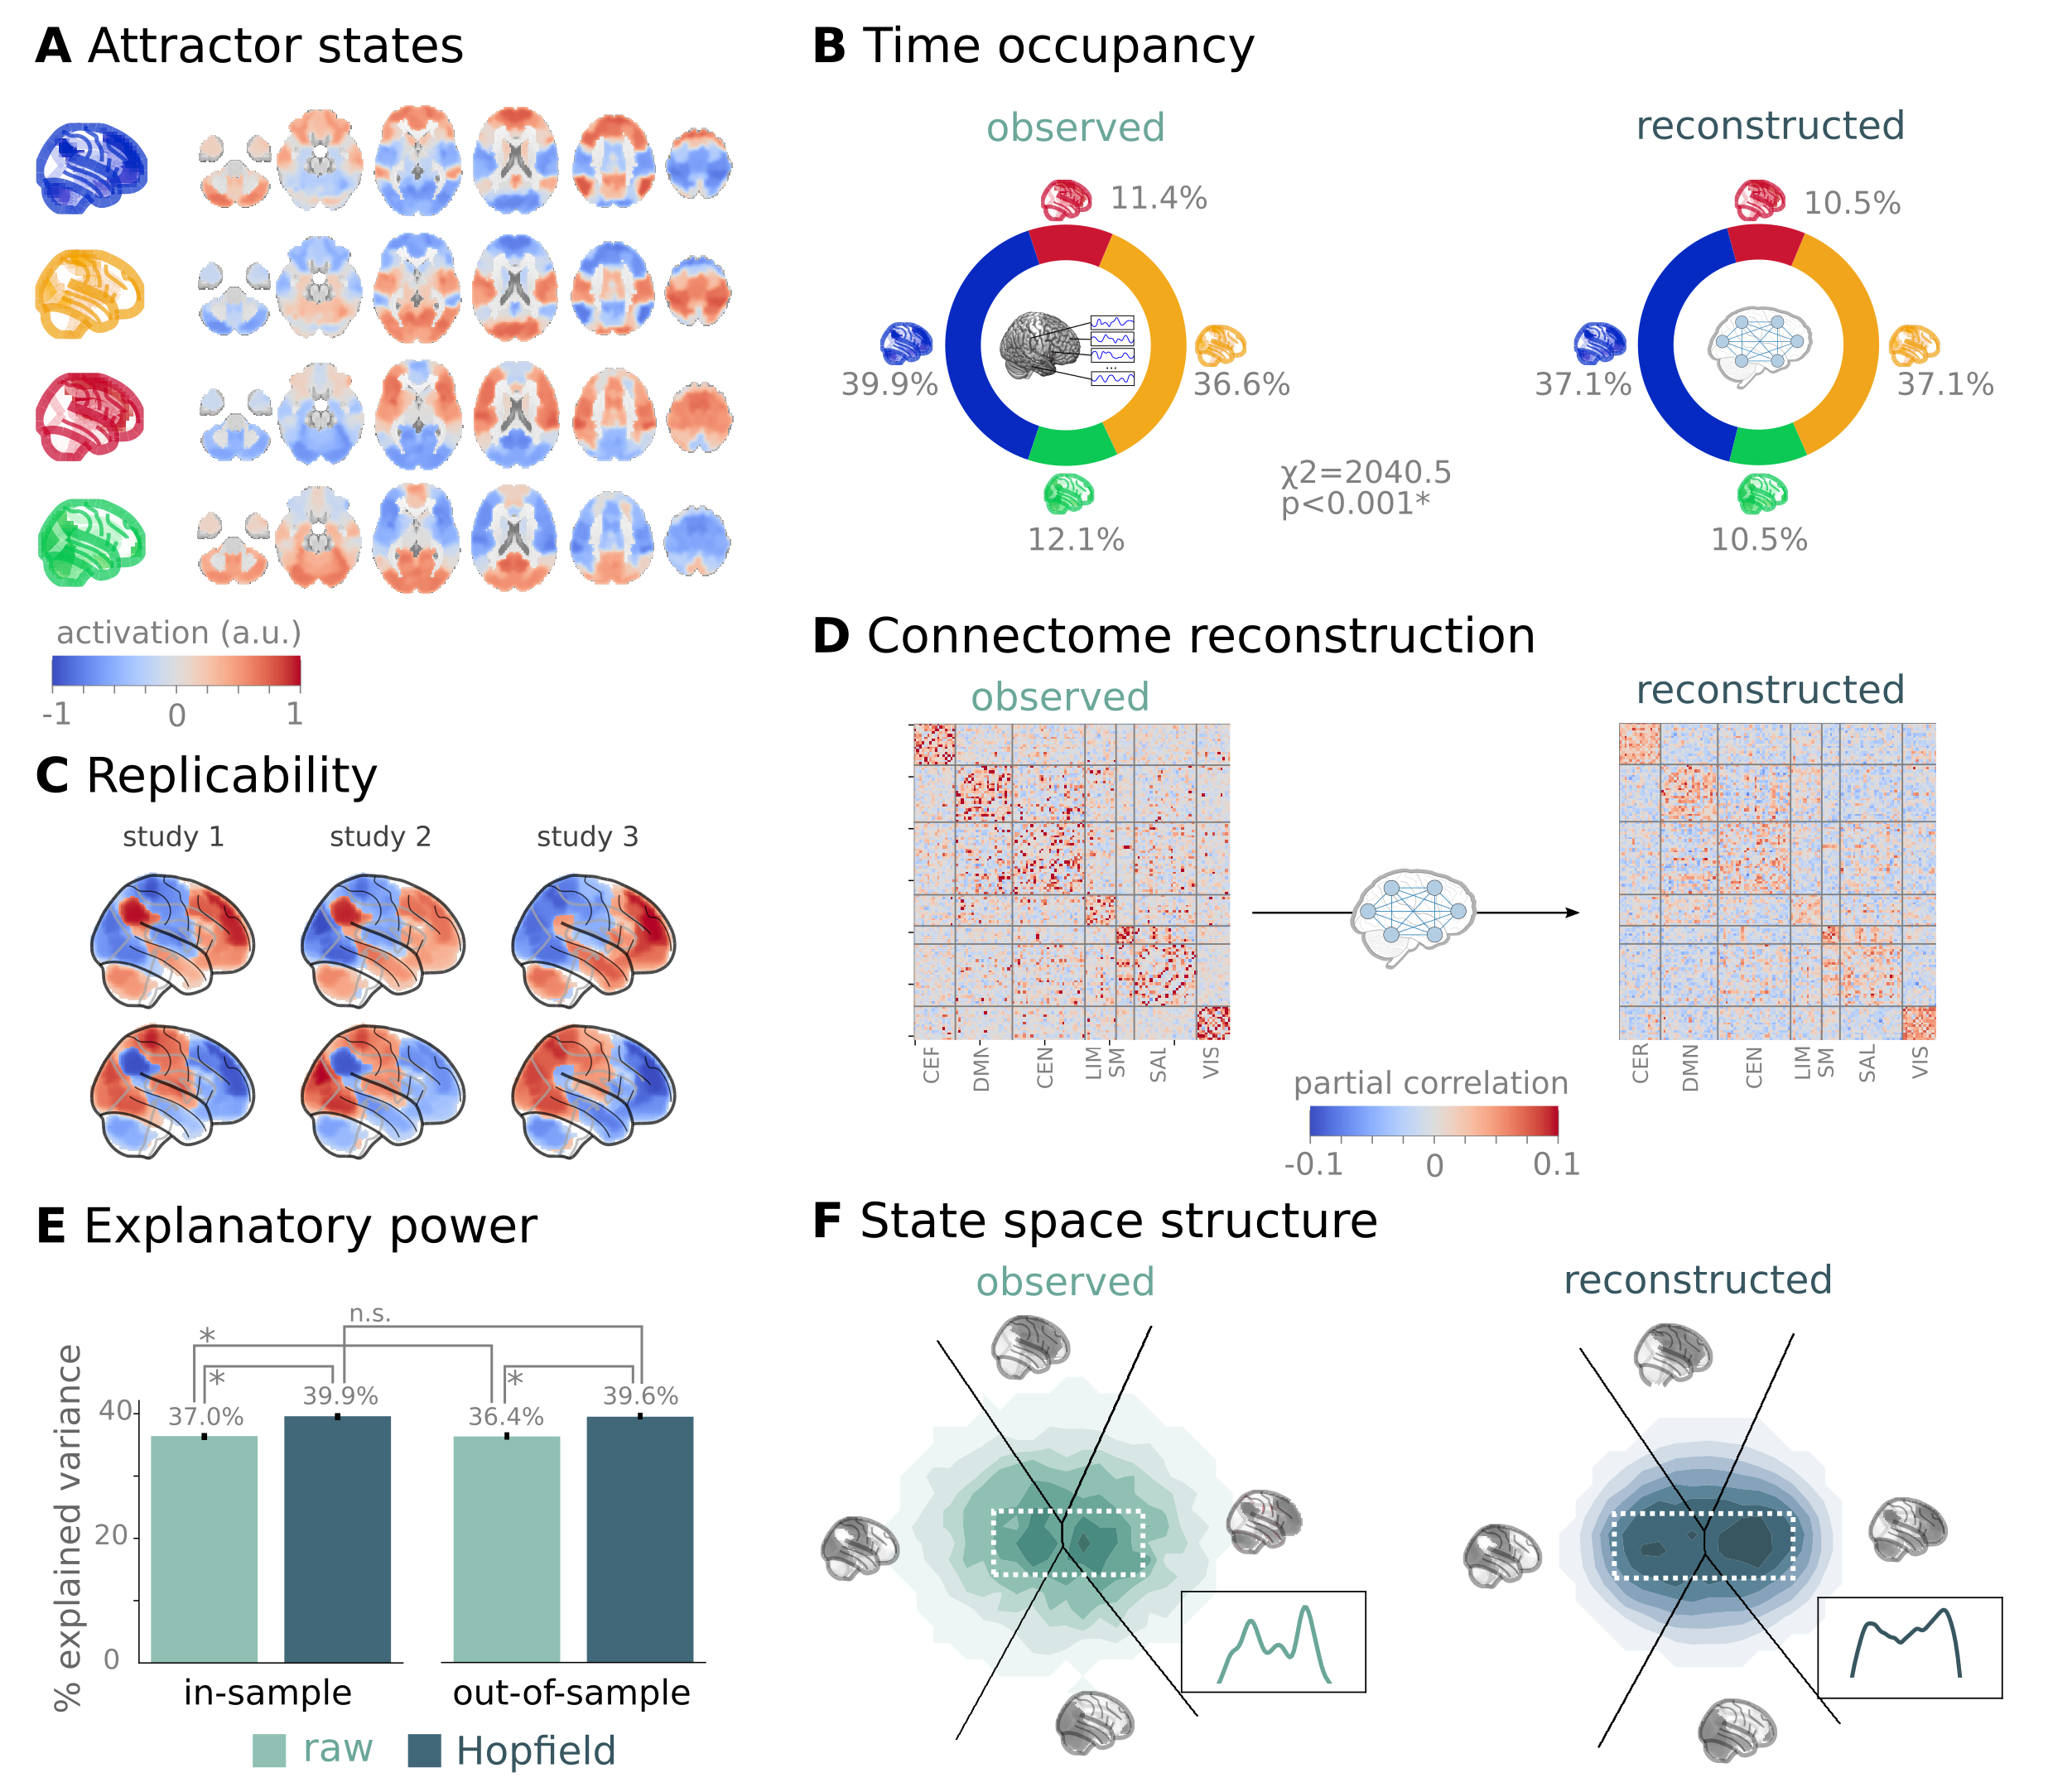
\includegraphics[width=0.7\linewidth]{files/face_validity-1e69675b824ba3957f117601f2f4ddee.png}
\caption[]{Empirical Hopfield-networks reconstruct real resting state brain activity.}
\label{rest-validity}
\end{figure}

Hopfield networks are known to exhibit remarkable robustness to noisy input (\href{https://doi.org/10.1073/pnas.79.8.2554}{}) and even to corrupted weights (\textbf{ref}). We found that this property renders connectome-based Hopfiled networks as a strikingly robust tool (Supplementary Analysis X), showing a remarkable replicability (mean Pearson's correlation \textbf{XX}) across the discovery datasets (study 1) and two independent replication datasets (study 2 and 3, Figure~\ref{rest-validity}C).

Further analysis in study 1 demonstrated that connectome-based Hopfield models very accurately reconstruct several characteristics of true resign state data.
First, the Hopfield projection explained a large amount of variance in the real resting state fMRI data in study 1 (mean $R^2=0.15$) and generalized well to study 2 (mean $R^2=0.13$) and study 3 (mean $R^2=0.12$) (Figure~\ref{rest-validity}E). Explained variance significantly exceeded that of a PCA performed on the real resting state fMRI data itself (Figure~\ref{rest-validity}E).

Second, during stochastic relaxation, the connectome-based Hopfield network spends three-quarter of the time on the basis of the first two attractor states (equally distributed across the two) and one-quarter on the basis of the second pair (again equally distributed). To test if this characteristic can also be found in real resting state data, we obtained normalized and cleaned mean timeseries in $m=122$ regions from all participants in study 1 obtained the attractor state of each time-frame via the connectome-based Hopfield network. We observed highly similar temporal occupancies to those predicted by the model ($\Chi^2$-test of equal occupancies: p\textless 0.00001, Figure~\ref{rest-validity}B).

Third, during the stochastic relaxation procedure, connectome-based Hopfield models generate regional timeseries that retain the partial correlation structure of the real functional connectome the network was initialized with, indicating a high-level of construct validity (Figure~\ref{rest-validity}D). To

Finally, our connectome-based Hopfield model also accurately reconstructs the bimodal distribution of the real resting state fMRI data on the Hopfield projection (Figure~\ref{rest-validity}F).

The ability of the connectome-based Hopfield model to reconstruct such characteristics of remarkable, given that the model was neither trained to reconstruct nor informed about any spatial (bi-model distribution, explanatory performance) or temporal patterns (temporal state occupancy) of the brain. The only information the model was provided with was the functional connectome, which was used to initialize the network and to constrain the dynamics of the network during stochastic relaxation. The fact that the model is able to reconstruct such characteristics of resting state brain dynamics, which are not explicitly encoded in the connectome, suggests that the connectome-based Hopfield model captures important relationships between the topology of brain connectome of the dynamics of the brain activation.

\subsection{An explanatory framework for task-based brain activity}\label{An explanatory framework for task-based brain activity}

The proposed framework provides a natural account for how activation patterns in the brain dynamically emerge form the underlying functional connectivity. To illustrate this, we obtained task-based fMRI data from a study by \href{https://doi.org/10.1371/journal.pbio.1002036}{} (study 4, n=33, see Figure~\ref{rest-validity}), invetsigating the neural correlates of pain, with focus on self-regulation.
We found that time-frames from obtained from periods with pain stimulation (taking into account hemodynamics, see Methods for details) locate significantly differently on the Hopfield projection than time-frames obtained from periods without pain stimulation (permutation test, p\textless 0.001, Figure~\ref{task-validity}A, left). Energies, as defined by the Hopfield model, were also significantly different between the two conditions (permutation test, p\textless 0.001), with higher energies during pain stimulation. The Hopfield-projections thus provide an intuitive account for how the underlying functional connectivity of the brain can give rise to different activation patterns, depending on the current input. Change in input (i.e. task) does not switch to the brain into a distinct mode of operation but acts as a perturbation of the system's dyanmics, resulting in mean activations changes that are only reliable measurable over an extended period of time, as done by conventional task-based fMRI analyses.

Participants were instructed to up- or down-regulate their pain sensation (resulting in increased and decreased pain reports and differential brain activity in the nucleus accumbens, NAc, see \href{https://doi.org/10.1371/journal.pbio.1002036}{} details), which resulted in further changes of the location of momentary brain states on the Hopfield-projection (permutation test, p\textless 0.001, Figure~\ref{task-validity}A, right). Interestingly, self-regulation did not manifest in significant energy changes (permutation test, p=0.36). This suggest that visualizong data on the Hopfiled projection can also capture changes in brain activity that originate from intrinsic modulation, rather than from changes in external input.

\begin{figure}[!htbp]
\centering
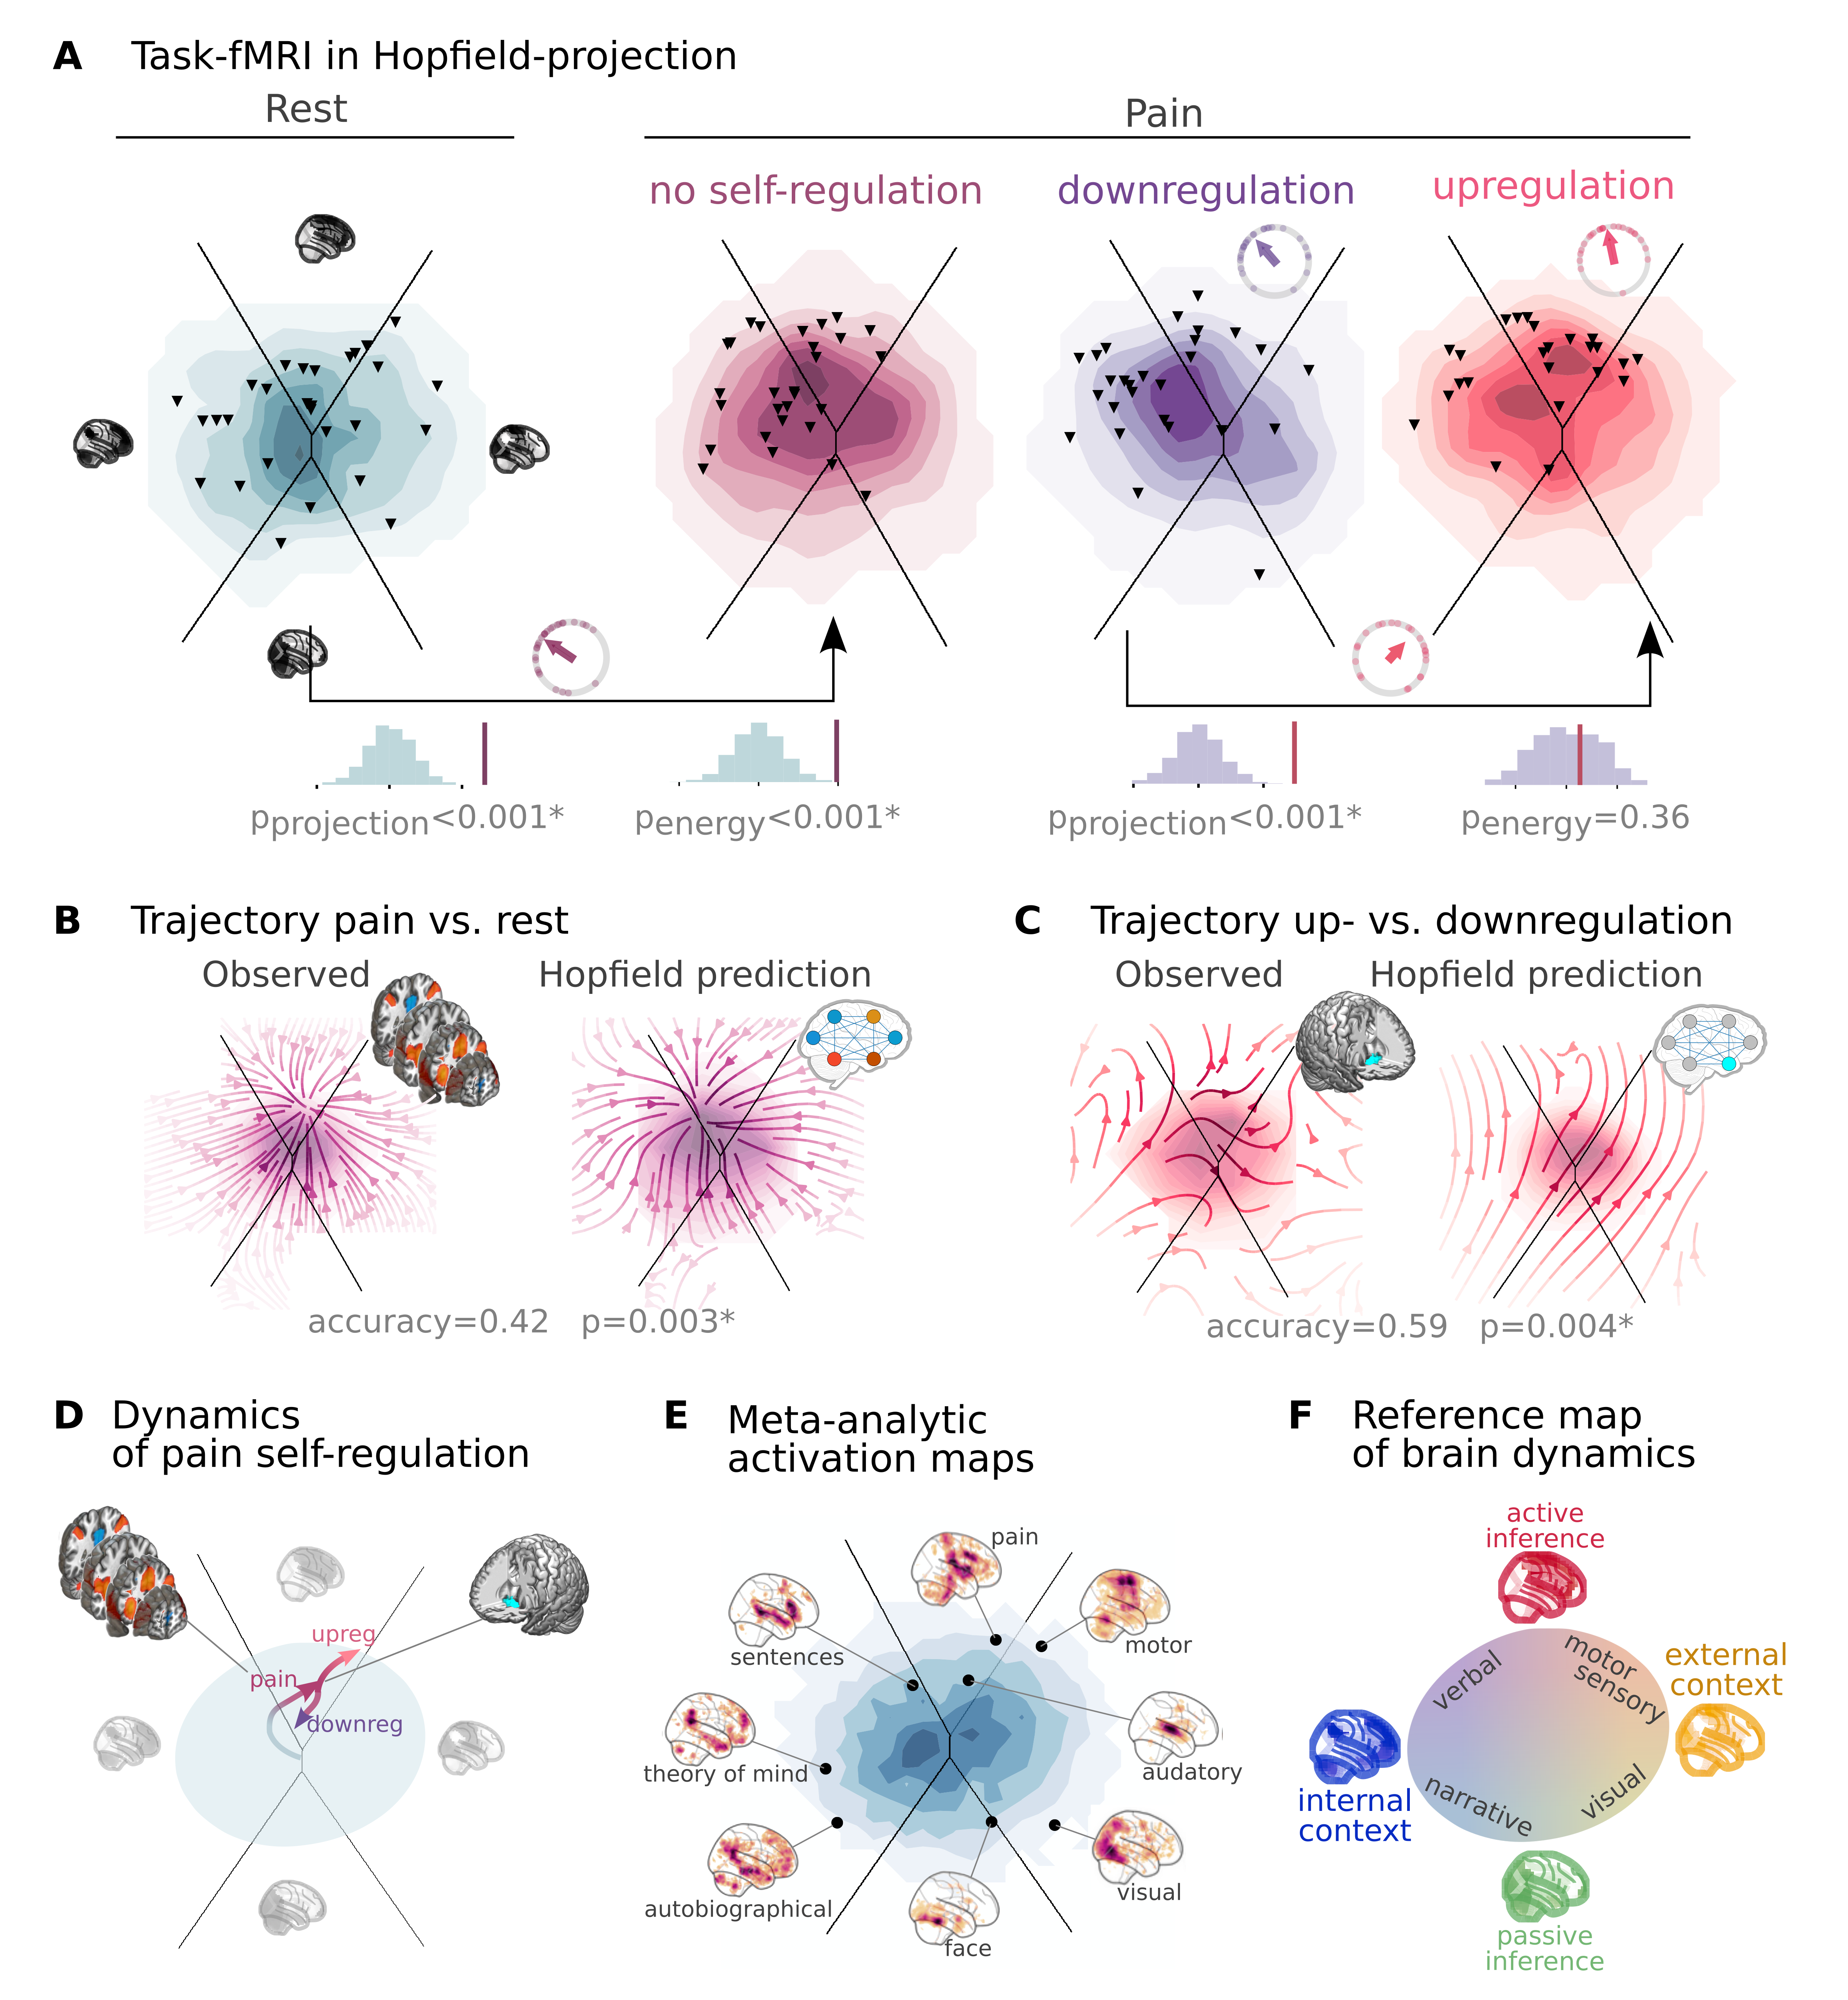
\includegraphics[width=0.7\linewidth]{files/task_validity-7f70e338ca1daa1874865999087b03c5.png}
\caption[]{Empirical Hopfield-networks reconstruct real task-based brain activity.}
\label{task-validity}
\end{figure}

The proposed framework offers much more than visualization and inference of resting state and task based data on the Hopfield projection.
It can provide a generative model for observed activity changes that can be used to predict brain activity under different conditions. To illustrate this, we used the Hopfield model to simulate brain activity during pain stimulation and self-regulation.
First we registered the frame-to-frame transitions in the real fMRI data (all four conditions: rest, pain without self-regulation, downregulation, upregulation) and converted those into the Hopfield embedding (resulting in a 2-dimensional vector on the Hopfield projection for each transition). Then, we assessed the mean direction in various segments of the projection (on a 6x6 grid). Next we took the difference of these mean directions between rest and pain (no regulation) (Figure~\ref{task-validity}B, left side), as well as between down- and upregulation (Figure~\ref{task-validity}C, left side). This analysis revealed remarkable non-linear trajectory patterns, showing the most likely direction the brain proceeds towards from a given state (activity pattern) in a given condition (pain without delf-regulation or upregulation), as compared to the reference state (rest and downregulation, respectively). In case of pain vs. rest, brain activity is pulled toward a "ghost attractor" located in the proximity of the Hopfiled projection typical pain activation map, as observed via conventional task-based fMRI analyses. In terms of attractor states, this belongs to the basin of attractor corresponding to sensory and motor processes (active inference). In case of up vs. downregulation, brain activity is pulled generally towards a similar direction, although with non-linear local perturbations and the lack of a clear ghost attractor.

Next, we aimed to assess, how much these non-linear dyanmics can be reconstructed by the proposed framework. To simulate how brain dynamics alter during pain stimulation, we obtained a meta-analytic pain activation map (\href{https://doi.org/10.1038/s41467-021-21179-3}{}) and introduced it with as additional signal on top of the Gaussian noise during the stochastic relaxation procedure. Not that, while adding such signal naturally results in a slight, linear shift on the Hopfield projection for each state generated during the stochastic relaxation procedure, that alone could only very weakly account for the observed nonlinear dyanmics in the real data (Supplementary material X). After optimizing across 5 different signal-to-noise (SNR) values (logarithmically spaced between 0.001 and 0.1) we found that, with a very low amount of signal added (SNR=0.01) the connectome-based Hopfield model is able to provide a highly accurate reconstruction of the observed non-linear differences in brain dynamics between the pain and rest conditions, including the "ghost attractor" of pain (Spearman's $\rho$ = 0.42, p=0.003, Figure~\ref{task-validity}B, right side).

Interestingly, the same model was also able to reconstruct the observed non-linear differences in brain dynamics between the up- and downregulation conditions (Spearman's $\rho$ = 0.59, p=0.004) with a very simple change; the addition (downregulation) or subtraction (upregulation) of activation in the NAc (the region in which \href{https://doi.org/10.1371/journal.pbio.1002036}{} observed significant chnages between up- and downregulation). Importantly, in this analysis, we did not have to optimize any paramters of the model, we simply used the same low SNR for the NAC that we already found optimal in the previous analysis (SNR=0.01, Figure~\ref{task-validity}C, right side).

These results provide a fresh perspective on the neural mechanisms beyond pain and its self-regulation and provides a mechanistic account for the role of both "traditional" pain-related regions and the NAc in pain regulation (Figure~\ref{task-validity}D). These results also highlight, that thr conceptual distinction between resting and task states might be - to a large degree - a false dichotomy. Rather, the brain is in a constant state of flux, which is only slightly perturbed by task states (even by so salient stimuli as pain) and the Hopfield projection can be used to visualize and quantify these dynamics.

To provide a comprehensive picture on how other tasks map onto the Hopfield projection, we obtained various task-based meta-analytic activation maps from Neurosynth (see Supplementary material X for details)  and plotted them on the Hopfield projection (Figure~\ref{task-validity}E). This analysis revealed that the Hopfield projection can be used to visualize and quantify the dynamics of a wide range of cognitive processes, including sensory, motor, cognitive and social processes and reveals that the two principal axes of the projection map well to internal vs. external context and active inference vs. passive perception, respectively.
In this coordinate system, visual processing is labeled "external-passive", sensory-motor processes "external-active", language, verbal cognition and working memory is labelled "internal-active" and long-term memory and autobiographic narratives fall into the "internal-passive" regime (Figure~\ref{task-validity}F). This analysis also revealed that the Hopfield projection can be used to visualize and quantify the dynamics of a wide range of cognitive processes, including sensory, motor, cognitive and social processes and reveals that the two principal axes of the projection map well to internal vs. external context and active inference vs. passive perception, respectively.

These results highlight a very powerful feature of the proposed generative framework, namely that it can be used to simulate and predict brain activity under different conditions. Predicting the effect of lower or higher level of activity in certain regions, or lower or higher connectivity among them, on global brain dynamics and responses to various tasks provides unprecedented opportunities for forecasting the effect of interventions, such as pharmacological or non-invasive brain stimulation, on brain function.

\subsection{Clinical relevance}\label{Clinical relevance}

In our final analysis, we provide a brief outlook towards the potential clinical applications of CBH analysis. We analyzed three large public clinical databases as provided by the Autism Brain Imaging Data Exchange (study 6: ABIDE, \textbf{ref}), the Centers of Biomedical Research Excellence (study 7: COBRE, \textbf{ref}) and the the Alzheimer's Disease Neuroimaging Initiative (study 8: ADNI, \textbf{ref}), analyzed resting state fMRI data of patients with autism spectrum disorder (ASD), schizophrenia (SCZ) and Alzheimer's disease (AD). Patients' data was contrasted to their respective control groups (typically developing controls for ASD, healthy control participants for SCH and individuals with mild cognitive impairment (MCI), respectively.

In all three datasets, we used the CBH model from study 1 and projected the fMRI timeseries of all involved participants onto the Hopfield projection. For each participant, we obtained the average activation of all time-frames belonging to the same attractor state (4 maps per participant) and compared these across groups with a permutation test, controlled for the family-wise error rate across brain regions and attractor states (122*4 comparisons).

We found several significant differences the mean attractor activation of patients as compared to the respective controls. In ASD, all four attractor activation maps showed significant differences (Figure~\ref{clinical-validity}A, \textbf{table}), characterized by altered activation in the \textit{precuneus, posterior congulate, sensory-motor system, posterior insula, and cerebellum}.

In SCZ, the most prominent differences were found in the subsystem for internal context, with elevated activity of regions that are not typically active in this state, including the \textit{thalamus, the striatum and several cortical regions} (Figure~\ref{clinical-validity}B, \textbf{table}). Additional activation increases in \textit{visual and motor} areas were observed in the active inference subsystem.

In the AD vs. MCI comparison, we found significant differences in two of the four attractor activation maps (Figure~\ref{clinical-validity}C, \textbf{table}), indicating changes in the resting state activity of subsystems for passive inference and internal context (both of which together host long-term memory processes, see Figure~\ref{task-validity}F). At the regional level, differences are characterized by altered activation in the \textit{dorsolateral prefrontal cortex (DLPFC) and the cerebellum}.

\begin{figure}[!htbp]
\centering

\includegraphics[width=0.7\linewidth]{files/state_analysis-792d79c1cf8a53d9d84001bf2e133f5f.svg}
\caption[]{Outlook: Empirical Hopfield-networks' clinical validity.}
\label{clinical-validity}
\end{figure}

\section{Discussion}\label{Discussion}

Regions of the brain are in a continuous process of exchanging information, resulting in co-activations commonly referred to as functional connectivity.
The amount of information exchanged is not constant across the brain but varies largely for various region pairs, spanning the complex network known as the functional connectome.
Here we have proposed a simplistic yet powerful model of how activity flow through this complex network topology naturally restricts the system's dyanmics, and gives rise to distinct brain sates and characteristic dynamic responses to perturbations.
In a series of experiments, we have shown that the proposed model can be used to accurately reconstruct and predict large-scale brain activity under different conditions, with unprecedented opportunities for forecasting the effect of interventions, such as pharmacological or non-invasive brain stimulation, on brain function.

The construct validity of our model is rooted in the activity flow principle, first introduced by \href{https://doi.org/10.1038/nn.4406}{}. The activity flow principle states that functional connectivity between region A and B can be conceptualized as the degree to which activity is transferred form A to B. This principle has been shown to successfully predict held out brain activations by a weighted sum of the activations of all the regions where the weights are set to the functional connectivity of those regions to the held-out region (\href{https://doi.org/10.1038/nn.4406}{}; \href{https://doi.org/10.1038/s41467-017-01000-w}{}; \href{https://doi.org/10.1371/journal.pbio.3001686}{}; \href{https://doi.org/10.1126/sciadv.abf2513}{}; \href{https://doi.org/10.1089/brain.2018.0586}{})).

\begin{quote}
ToDo: latent FC-based modelling: \href{https://doi.org/10.1162/netn\_a\_00234}{}
\end{quote}

Our model was born from the intuition that the recurrent, iterative application of the activity flow equation results in a system showing close analogies with a type of recurrent artificial neural networks, know as Hopfiled networks (\href{https://doi.org/10.1073/pnas.79.8.2554}{}).
Hopfield networks have previously been shown to exhibit a series of characteristics that are also highly relevant for brain function, including the ability to store and recall memories (\textbf{ref}), self-repair (\textbf{ref}), a staggering robustness to noisy or corrupted inputs (\textbf{ref}) and the tendency to produce multistable dynamics organized by the "gravitational pull" of a finite number of attractor states (\textbf{ref}).

The proposed link between activity flow and Hopfield networks has and important implication: network weights must be initialized with functional connectivity values, (specifcally, partial correlations, as recommend by \href{https://doi.org/10.1038/nn.4406}{}), instead of applying an explicit training procedure (common in the "neuroconnectomist" approach (\textbf{ref})) or using the structural connectome (a standard practice of conventional computational neuroscience (\textbf{ref})).

Using functional conncetome-based Hopfield (CBH) model provides a simple yet powerful framework for the mechanistic understanding of brian dynamics. Its simplicity comes with an important advantages.

First, increasing model complexity results in an exponential explosion of the parameter space. Although complex, fine-grained computation models hold promise a full-blown understanding, they very easily overfit real data (\textbf{ref}). The basic CBH approach has only two hyperparameters (temperature and noise) and produce fairly consistent behavior on a wide range of parameter values. To demonstrate the power of simplicity, in the present work, we deliberately minimized fine-tuning of any free parameters. We fixed the temperature parameter at a value that robustly provides 4 attractor states and used a single noise level for all experiments (selected with a coarse optimization procedure to approximately mimic the distribution of real data).

Second, increasing complexity means increasing burden in terms of interpretability. The CBH model establishes a simple, direct link between two most popular measures of brain function: functional connectivity and brain activity. This link is not only conceptual, but also mathematical, and allows us to investigate and forecast changes of the system's dyanmics in response to perturbations of both activity and connectivity.

In this initial investigation, we further reduced complexity by restricting the analysis to a simplified 2-dimensional embedding of the state-space generated by the CBH approach, which we refer to as the Hopfield projection. This projection is a powerful tool for the visualization of the CBH model's dynamics, and allows for a direct comparison with the dynamics of the original brain activity.

However, the Hopfield projection only conveys a small proportion of the richness of the full state-space dynamics reconstructed by the CBH model.
Investigating higher-dimensional dynamics, fine-tuned hyperparameters, the effect of different initializations and perturbations is an important direction for future work, with the potential to further improve the model's accuracy and usefulness.

Given these intentional simplifications, it is remarkable, if not surprising, how accurately the CBH model is able to reconstruct and predict brain dynamics under a wide range of conditions. Next to accurately reconstructing the distribution of, and the time spent in, different brain states during resting state, its superiority in explaining, and generalizing to, resting state brain activation patterns over principal components derived from the same data is particularly striking.
The question arises, how can a relatively simple model, which is informed about empirical brain dynamics only through the functional connectome, be so powerful?
A possible answer is that, while empirical data (and its principal components) are corrupted by noise and low sampling rate,
the highly noise tolerant nature and the self-repair properties of the CBH architecture allow it to capture and reconstruct the basic principles of the underlying dynamics.

The noise-tolerance of the proposed architecture also explains the high replicability of CBH attractors across different datasets (study 2 and 3).
The observed level of replicability allowed us to re-use the CBH model constructed with the connectome of study 1 for all subsequent studies, without any further fine-tuning or study-specific parameter optimization.

The connectome obtained form study 1 was also used to evaluate the model's ability to capture and forecast task-induced brain dynamics in study 4 and 5. In these analyses, was not only able to capture participant-level activity changes induced by pain and self-regulation (showing significant differences on the Hopfield projection and in terms of state energy) but also accurately predicted the non-linear changes in activity flow induced by activity changes characteristic.

Brain dynamics can not only be perturbed by task or other types of experimental or naturalistic interventions, but also by pathological alterations.
In our analysis of clincial sampples study 6-8 we found that mean attractor activations show characteristic alteration in autism spectrum disorder (ASD), Schizophrenia (SCH) and Alzheimer's disease (AD). These changes were also detectable on the Hopfield projection, and were accompanied by significant changes in the state energies.
The Hopfiled projection also allowed us to visualize the effect of different types of perturbations on the brain's attractor landscape, providing a novel perspective on the pathophysiology of these disorders.

\begin{quote}
ToDo: more details
\end{quote}

Together, these results open up a series of exciting opportunities for the mechanistic understanding of brain function. By its generative nature, the CBH model could foster analyses that aim at disentangling causal relationships, which are extremely difficult to infer in case of systems as complex as the brain. It could, for instance, aid the differentiation of primary causes and secondary effects of particular activity or connectivity changes in various clinical conditions.

Moreover, the CBH approach might provide testable predictions about the effects of interventions, like pharmacological or non-invasive brain stimulation (e.g. transcranial magnetic or direct current stimulation, focused ultrasound) or neurofeedback, on brain function.
For instance, in the context of pain, the CBH model might be used to predict the effect of various analgesic drugs (or other treatment strategies with known neural correlates) on the individual level (e.g. based on the individual functional connectome).
Aidng the design of personalized medicine approaches is a particularly promising field of application for the proposed framework.

The generative nature of the proposed framework may be also used to generate synthetic brain activity data, which can be used to train and test machine learning algorithms, such as deep neural networks, for the prediction of brain activity from functional connectivity. This approach may be particularly useful in the context of clinical applications, where the amount of available data is often limited.

\section{Conclusion}\label{Conclusion}

To conclude, here we have proposed a novel computational framework that accurately captures and predicts brain dynamics under a wide range of conditions.
The framework models large-scale activity flow in the brain with a recurrent artificial neural network architecture that, instead of being trained to solve specific tasks or mimic certain dynamics, is simply initialized with the empirical functional connectome. The framework identifies biologically meaningful attractor states and provides a model for how these restrict brain dyanmics.
The proposed framework, referred to as the connectome-based Hopfield (CBH) model, can accurately reconstruct and predict brain dynamics under a wide range of conditions, including resting state, task-induced activity changes, and pathological alterations.
CBH analyses provide a simple, robust, and highly interpretable computational alternative to the conventional descriptive approach to investigating brain function and establish a link between connectivity and activity.
The generative nature of the proposed model opens up a series of exciting opportunities for future research, including novel ways of assessing causality and mechanistic understanding and the possibility to predict the effects of various interventions, thereby paving the way for novel personalized medical approaches.

\section{Methods}\label{Methods}

\begin{table}
\centering
\begin{tabular}{p{\dimexpr 0.143\linewidth-2\tabcolsep}p{\dimexpr 0.143\linewidth-2\tabcolsep}p{\dimexpr 0.143\linewidth-2\tabcolsep}p{\dimexpr 0.143\linewidth-2\tabcolsep}p{\dimexpr 0.143\linewidth-2\tabcolsep}p{\dimexpr 0.143\linewidth-2\tabcolsep}p{\dimexpr 0.143\linewidth-2\tabcolsep}}
\toprule
study & modality & analysis & n & age (mean$\pm$sd) & \%female & references \\
\hline
study 1 & resting state & discovery & 41 & 26.1$\pm$3.9 & 37\% & \href{https://doi.org/10.1038/s41467-019-13785-z}{} \\
study 2 & resting state & replication & 48 & 24.9$\pm$3.5 & 54\% & \href{https://doi.org/10.1038/s41467-019-13785-z}{} \\
study 3 & resting state & replication & 29 & 24.8$\pm$3.1 & 53\% & \href{https://doi.org/10.1038/s41467-019-13785-z}{} \\
study 4 & task-based & pain self-regulation & 33 & \begin{quote}
todo
\end{quote}

 & \begin{quote}
todo
\end{quote}

 & \href{https://doi.org/10.1371/journal.pbio.1002036}{} \\
study 5 (Neurosynth) & task-based & coordinate-based meta-analyses & 14371 studies in total & \textbullet~~\newline
 & \textbullet~~\newline
 & \href{https://doi.org/10.3389/conf.fninf.2011.08.00058}{} \\
study 6 (ABIDE) & resting state & Autism Spectrum Disorder & ASD: 98, NC: 74 & \begin{quote}
todo
\end{quote}

 & \begin{quote}
todo
\end{quote}

 & \begin{quote}
todo
\end{quote}

 \\
study 7 (ADNI) & resting state & Alzheimer's Disease vs. Mild Cognitive Impairment & AD:, MCI: & \begin{quote}
todo
\end{quote}

 & \begin{quote}
todo
\end{quote}

 & \begin{quote}
todo
\end{quote}

 \\
study 8 (COBRE) & resting state & Schizophrenia & SCH: , HC: & \begin{quote}
todo
\end{quote}

 & \begin{quote}
todo
\end{quote}

 & \begin{quote}
todo
\end{quote}

 \\
\bottomrule
\end{tabular}
\end{table}

\subsection{Hopfield network}\label{Hopfield network}

The weights $w_{ij}$ have to be symmetric and the diagonal elements are set to zero.

Todo

Todo



\bibliographystyle{unsrtnat}
\bibliography{main.bib}

\end{document}
